\documentclass[tikz,border=10pt]{standalone}
\begin{document}
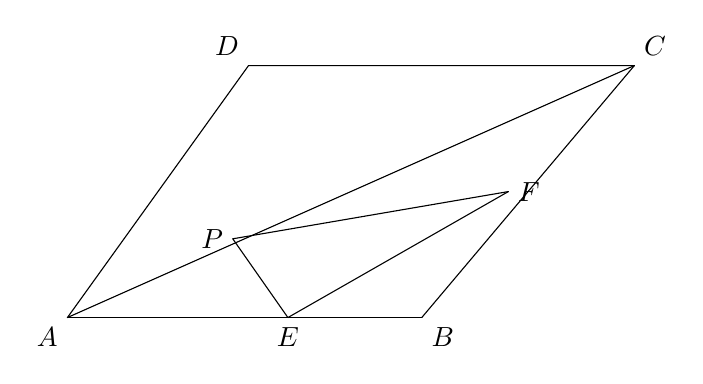
\begin{tikzpicture}[line cap=round,line join=round,scale=1]

\coordinate (A) at (0,0);
\coordinate (D) at (2.3,3.2);
\coordinate (C) at (7.2,3.2);
\coordinate (B) at (4.5,0);
\coordinate (E) at (2.8,0);
\coordinate (P) at (2.1,1.0);
\coordinate (F) at (5.6,1.6);

\draw (A) -- (D) -- (C);
\draw (A) -- (B);
\draw (B) -- (C);

\draw (A) -- (C);
\draw (P) -- (F);
\draw (P) -- (E);

\draw (E) -- (F);

\node[below left] at (A) {$A$};
\node[above left] at (D) {$D$};
\node[above right] at (C) {$C$};
\node[below right] at (B) {$B$};
\node[below] at (E) {$E$};
\node[left] at (P) {$P$};
\node[right] at (F) {$F$};

\end{tikzpicture}
\end{document}
